\newpage
\section{Camera Calibration}
Ever since the lens was introduced, subsequently replacing the pinhole camera, a way of performing calibration of a camera was needed. When the somewhat odd shape of the lens is utilized to increase the amount of light in the captured image, distortions can occur. There are primarily two types of distortion: radial and tangential distortion.
\subsection{Distortion and camera parameters} \label{theory:cameracalib}
In modern cameras with zoom lenses, radial distortion is the most common one. Radial distortion can result in either a pin-cushion or barrel distortion effect, as can be seen in figure \ref{fig:lensdistortiongraphic}.
\begin{figure}[h]
    \centering
    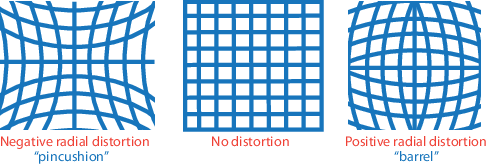
\includegraphics[width=0.8\textwidth]{figures/CameraCalibration/calibration_radial_distortion.png}
    \caption{Visualizing pin-cushion and barrel effect. \cite{lensdistortiongraphic}. Input to system is a rectangular grid as seen from the middle image.}
    \label{fig:lensdistortiongraphic}
\end{figure}
As visualized in the figure, this effect would be most prominent at the edges of the image. As the zoom level of the lens increases, the distortion effect increases too, often also because more of the camera frame is used to show important information. Barrel distortion often occurs when using wide-angle lenses. 
Tangential distortion makes the image looks stretched and tilted and often happens when the camera sensor is held at an angle with respect to the camera lens. This effect should not occur in most modern cameras. \\

Luckily, these distortion effects can be mitigated with some calibration. 


Combining the knowledge of a pin-hole camera model from section \ref{reconstruction:cameramodels} and the distortion, a relatively simple calibration can be done. The pin-hole camera model will be used for converting between the real world and camera coordinates. The pin-hole model does not include a lens, so by modeling and removing the distortion, the effect of the lens is included in the calibration. 

Only four equations are needed to model the radial and tangential distortion in $x$ and $y$ \cite{OpenCVCameraCalibrationTutortial}:
\begin{align}
    x_{distorted,\; radial} &= x\left(1+k_1r^2 + k_2r^4 + k_3 r^6\right) \\
    y_{distorted, \;radial} &= y\left(1+k_1 r^2 + k_2 r^4 + k_3r^6\right) \\
    x_{distorted, \; tangential} &= x + \left( 2p_1xy + p_2(r^2 + 2x^2) \right) \\
    y_{distorted, \; tangential} &= y+ \left(p_1(r^2 + 2y^2) + 2p_2xy \right)
\end{align}

The coefficients for the distortion are $distortion\_coefficients \;= \;[k_1, \; k_2, \; p_1, \; p_2, \; k_3 ]$. The $k$'s describe radial factors, and the $p$'s describe tangential factors. So for a given set of undistorted coordinates $(x,y)$, the distorted coordinate set can be calculated, for either radial or tangential distortion. In most scenarios, only the radial distortion is present. Furthermore, the first distortion coefficient used in the lower order term is often sufficient.\\

In order to map the world 3D coordinate system to the 2D image plane, a 3x4 matrix describing the relation between the two is needed, denoted $P$. 


It consists of one 3x3 matrix containing details about the pin-hole camera model, denoted $K$ and one 1x3 vector containing information about translation and rotation of the camera, denoted $ R $ and $t$. 
\begin{equation}
   w\left[\begin{array}{c}
u \\
v \\
1
\end{array}\right]=P\left[\begin{array}{c}
X \\
Y \\
Z \\
1
\end{array}\right],
\hspace{1cm} P = K[R \mid t] 
\end{equation}

%\begin{equation}
%w\;[u\;v \;1]=[X \;Y \;Z \;1] \;P \:\:, \:\:\:\:\:
%P = \left[\begin{array}{l}
%\mathrm{R} \\
%\mathrm{t}
%\end{array}\right] \mathrm{K}
%\end{equation}

$w$ is a scaling factor. $u,\; v$ are the pixel coordinates, and $X,\;Y,\;Z$ are world coordinates. $w$ arise from the use of homography to relate a 2D image plane to a 3D world space.\\

The 3x3 matrix $K$ is the intrinsic parameters, and describe the optical center and focal lengths. The 3x3 matrix $R$ and the 1x3 vector $t$ are the extrinsic parameters, and describe the location of the camera in the 3D world. 
In eq. \ref{eq:cameramatrix}, the system is written as two separate matrices, only using the intrinsic parameters. This assumes the $X, \; Y,\;Z $ is already translated to camera coordinates using the extrinsic parameters.
\begin{equation}
\left[\begin{array}{l}
u \\
v \\
w
\end{array}\right]=\left[\begin{array}{ccc}
f_{x} & 0 & c_{x} \\
0 & f_{y} & c_{y} \\
0 & 0 & 1
\end{array}\right]\left[\begin{array}{l}
X \\
Y \\
Z
\end{array}\right]
\label{eq:cameramatrix}
\end{equation}
The matrix, $K$, containing the intrinsic parameters, will from here on be denoted as the camera matrix. \\


For this use case, the real parameters of interest are the intrinsic, extrinsic, and first radial distortion parameters. When doing the calibration, this is exactly what is found. The parameters are found by taking images of a specific pattern of known dimension and going through a few steps of equations to derive the values of interest. This will be described a bit more in the following paragraph. The patterns are typically either a chessboard pattern or a circle grid. There are more complex types of calibration patterns as well, but these won't be considered.\\


 About 10 to 15 images of the calibration pattern should yield a good result according to OpenCV documentation. It is important to note, that if any settings on the camera change (i.e. zoom is changed slightly), the calibration must be redone as the parameters have changed.\\ 


To do the calibration, a chessboard pattern will be used as a calibration pattern. The number of grid corners in the horizontal and vertical direction is specified, as well as the size of each square. The numbers of rows are even, and the number of columns is odd to ensure no rotation ambiguity.\\ 


In order to extract the chessboard corners, the built-in function of OpenCV appropriately named "FindChessboardCorners" will be used \cite{findchessboardcornersOpenCV}. This was chosen to limit the time spent on calibration to focus on the main problems of the project. 

This function detects the chessboard corners of a specified grid dimension. 
%The method is based on a paper by A. Duda and U. Frese \cite{AlgoForChessBoardDetection}.\\ 
The function finds all the corners and maps them so you end up with points in 3D space having corresponding points in the 2D image plane. The method works by doing adaptive erosion and thresholding, which binarizes the image and separates the white and black squares nicely into connected quadrilaterals. Afterward, there is done refinement on the pixels found using the function "cornerSubPix", which does refinement of the found corners. It uses image gradients, and least-squares optimization to find the corners \cite{AlgoForChessBoardDetection}. \\

When the chessboard corners have been found, the intrinsic and extrinsic parameters can be estimated. The estimation is done using the "Camera Calibration" function of OpenCV \cite{calibrateCameraOpenCV}. The method it carries out is based on the previous work of others and is cited in the documentation for the function. Briefly described, the algorithm performs 3 different steps: 1) compute initial values of the intrinsic parameters, 
2) estimate camera pose by using the set of corresponding points from the chessboard detection and the initial value of intrinsic parameters, 
3) do global optimization using Levenberg-Marquardt, in order to minimize reprojection error between the corresponding points. After this is done, a set of intrinsic and extrinsic values are computed, and the calibration is done.\\ 


These newfound values can then be used to undistort images, or derive more information about the camera in 3D world coordinates, to ie. find the focal length in mm. This will be explored in the following section.


% Maybe this belongs in another section
\subsection{Evaluation of the camera calibration} \label{tests:cameracalib}
The relevant code to do camera calibration has been implemented accordingly in C++ using OpenCV. The code can be found in appendix \ref{appendixA}. The same settings for the camera that was used for data collection will also be used for calibration. This is crucial, or else the resulting calibration changes.\\ 

As mentioned earlier, a chessboard pattern will be used for calibration. Because the data collection was done by recording a video of the rotating object, the calibration will also be done using video. Screenshots of the video where the calibration pattern is in focus will be extracted manually and used for the calibration. Either the pattern or the camera needs to be fixated. The other part is then moved around, to capture different angles of the calibration pattern.\\ 

It is necessary to use video recording when doing the calibration instead of regular photos, because the dimensions and resolution of the images change between video recording and regular capture mode, resulting in completely different calibrations.\\

The calibration pattern was fixed on the wall, and the camera was moved around to different angles. A few example images can be seen below in figure \ref{fig:calib_1} and \ref{fig:calib_2}.
\begin{figure}[h!]
    \centering
    \begin{minipage}[t]{0.48\textwidth}
        \centering
        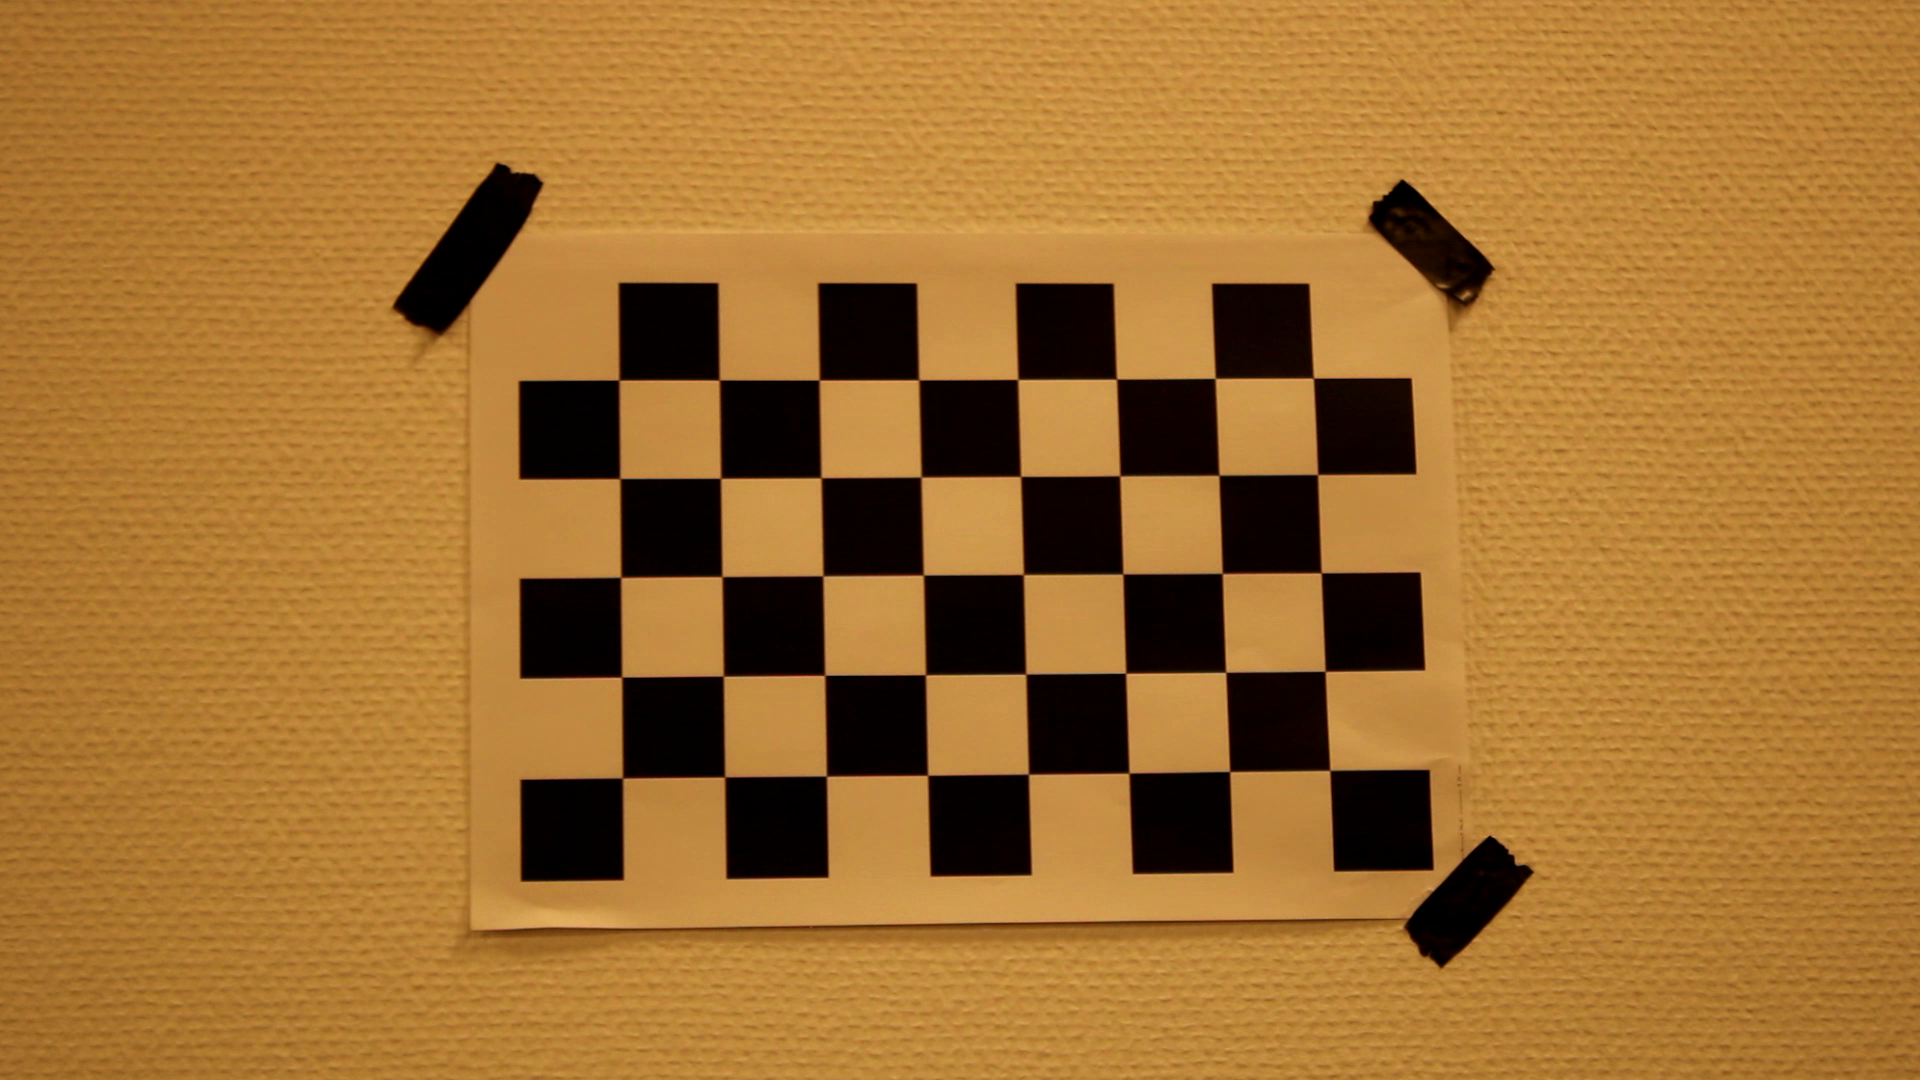
\includegraphics[width=0.95\textwidth]{figures/CameraCalibration/im1.png}
        \caption{Screenshot from calibration video, pattern is centered.}
    \label{fig:calib_1}
    \end{minipage}%
    \hspace{.03\textwidth}
    \begin{minipage}[t]{0.48\textwidth}
        \centering
        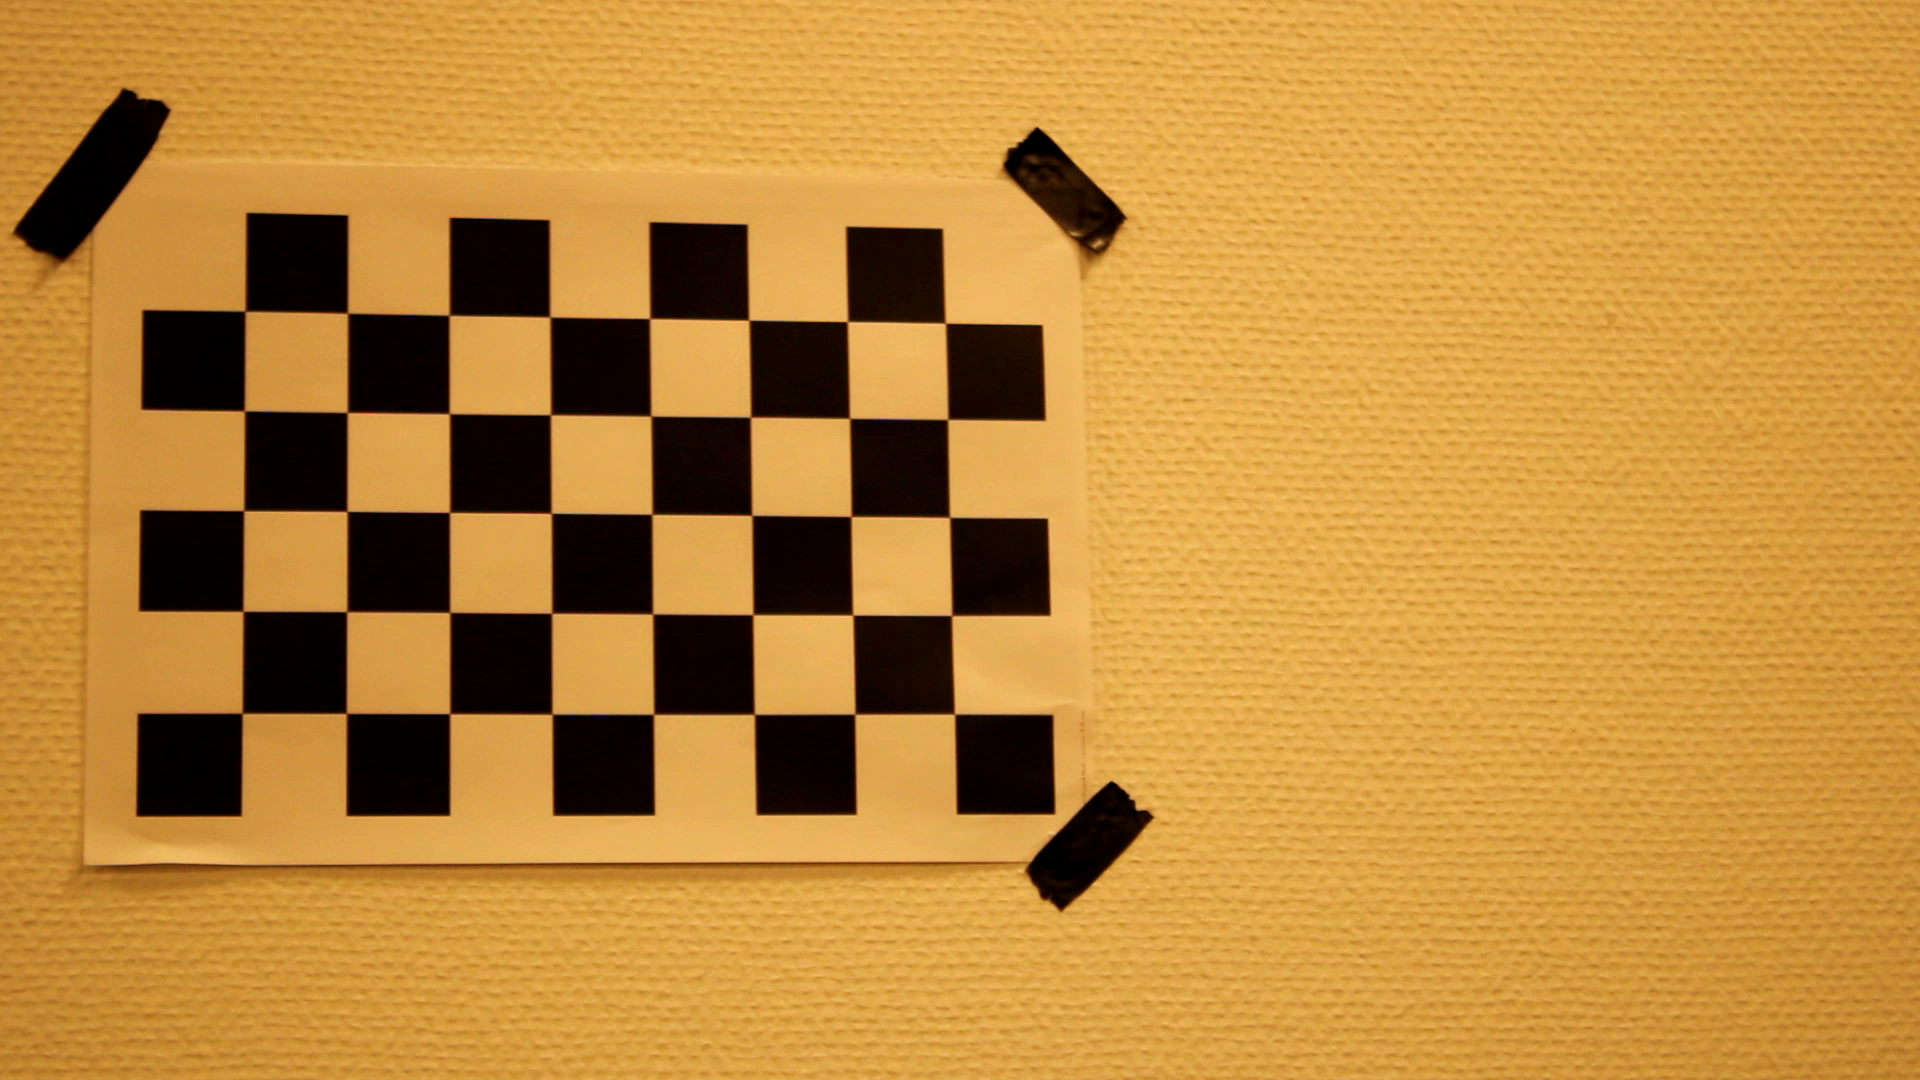
\includegraphics[width=0.95\textwidth]{figures/CameraCalibration/im6.png}
        \caption{Screenshot from calibration video, pattern is off-center to the left}
        \label{fig:calib_2}
    \end{minipage}
\end{figure}

In figure \ref{fig:calibpattern1marked}, the result of what the function "FindChessboardCorners" found is plotted. As is visible, only the inner part of the grid is localized. This is because the function only looks at where the black squares intersect with each other. 
\begin{figure}[h]
    \centering
        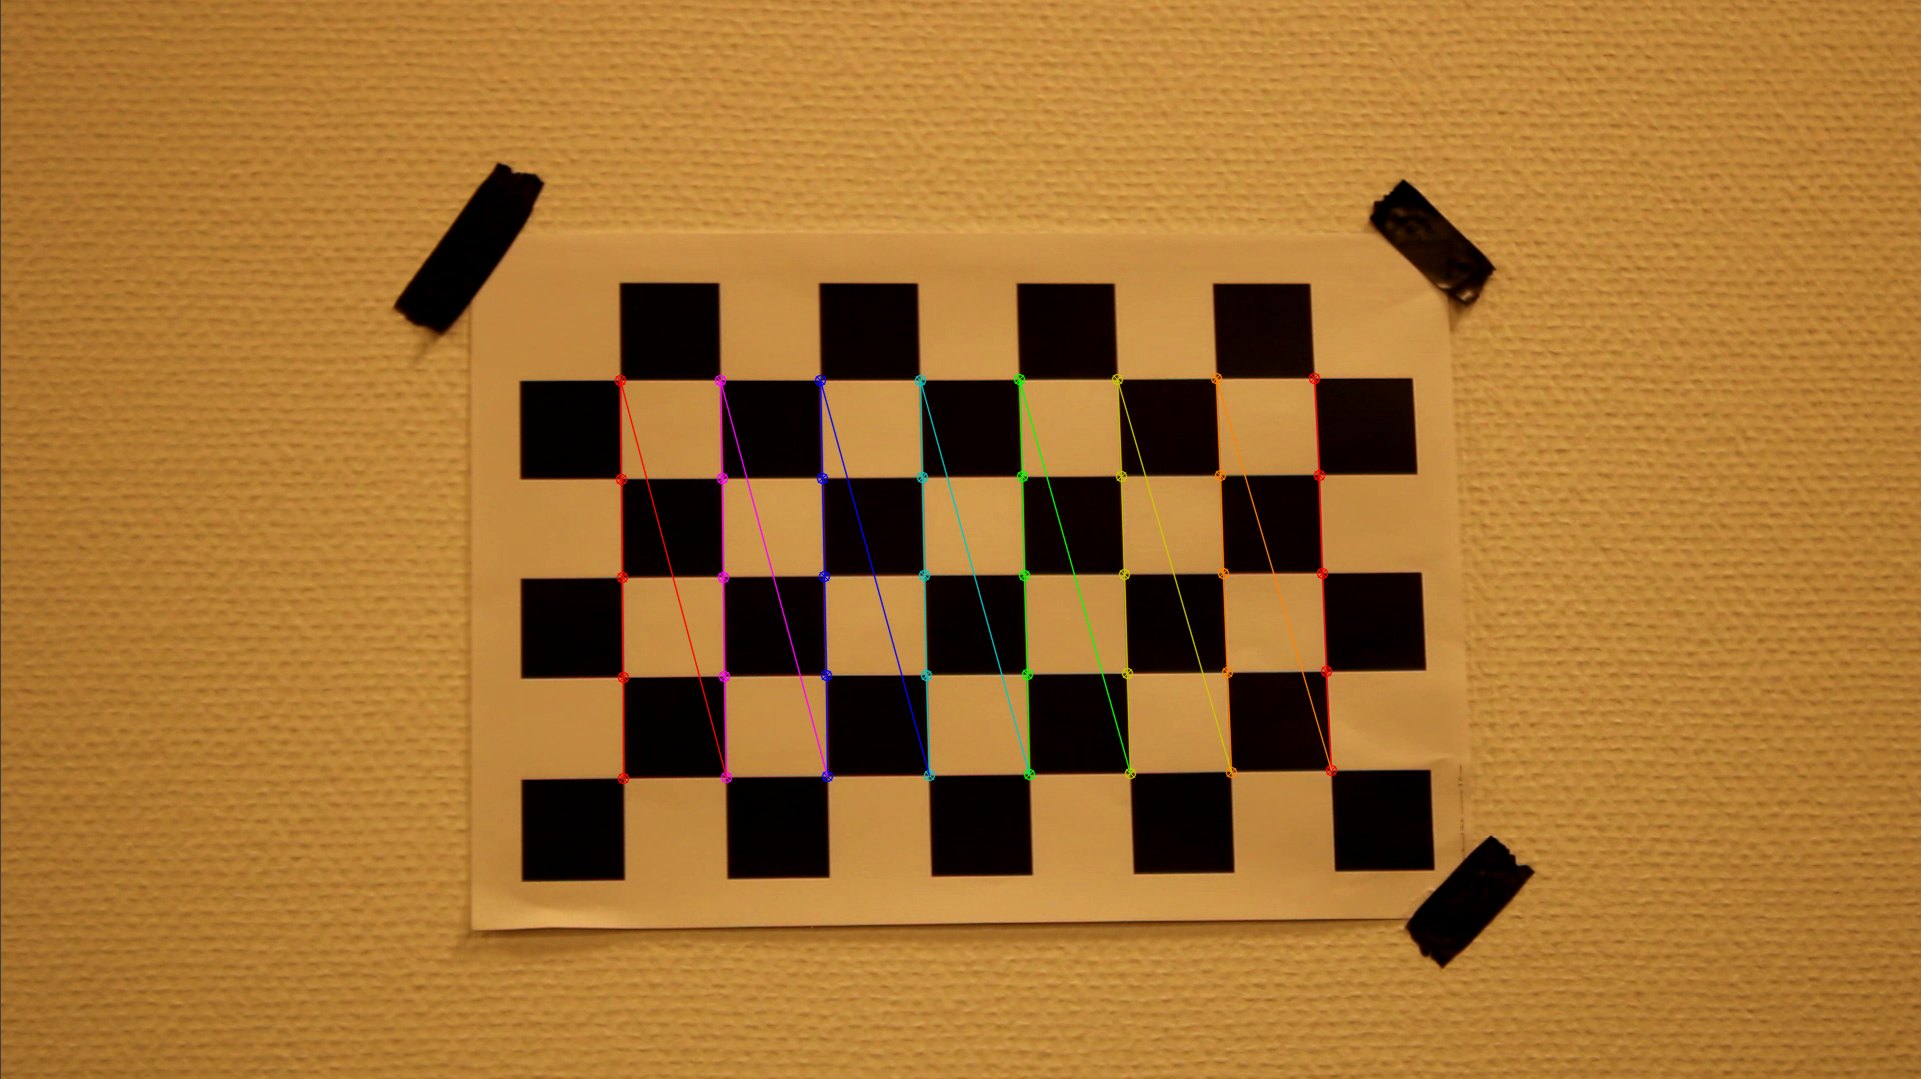
\includegraphics[width=0.95\textwidth]{figures/CameraCalibration/im1_marked.png}
        \caption{Screenshot from calibration video, pattern is centered, with result of the FindChessboardCorners function. }
    \label{fig:calibpattern1marked}
\end{figure}
This was done for all photos that was used for the calibration. It took a few tries to get images where the function could find the patterns, without resizing the images or adjusting the zoom (and thus changing the result of the calibration entirely).\\ 

In section \ref{result:cameracalib}, the coefficients of the calibration and the undistortion will be examined. 





\subsection{Results} \label{result:cameracalib}
From the calibration, the distortion coefficients and the camera matrix is of primary interest. The calibration was performed as described in section \ref{theory:cameracalib}, and the resulting camera matrix is found in eq. \ref{eq:cameramatrixvals}, and the distortion coefficients in eq. \ref{eq:distortcoeff}.
\begin{equation}
\text{Camera matrix: }\boldsymbol{K} = \left[\begin{array}{ccc}
4803.75 & 0 & 903.487 \\
0 & 4794.07 & 409.888 \\
0 & 0 & 1
\end{array}\right]
\label{eq:cameramatrixvals}
\end{equation}
\begin{equation}
    \text{Distortion coefficients: [0.14673, -1.40272, -0.01022, -0.00410, 37.0259]} 
    \label{eq:distortcoeff}
\end{equation}

The optical center seems slighty skewed in y coordinate considering that the resolution of the recording is 1920x1080. The focal length in x and y are very similar as expected since the pixels in the sensor of the camera are close to square. \\
%Calculating the focal length in world coordinates using equations described in section \textbf{INSERT WHICH SECTION THIS IS DESCRIBED IN}, the lengths are found as: $f_x = 55.7936\;[mm]$ and $f_y = 66.1404 \;[mm]$. According to the camera, the focal length was in fact 55 mm, so the calibration must be decent. \todo{section about focal length needs to be fixed}\\

Using the newly found distortion coefficients, the undistortion can be performed. 
After completing the undistortion, the images only change slightly. This can be seen in figure \ref{fig:calibpattern1undistorted} for the same image used section \ref{tests:cameracalib}.
\begin{figure}[h!]
        \centering
        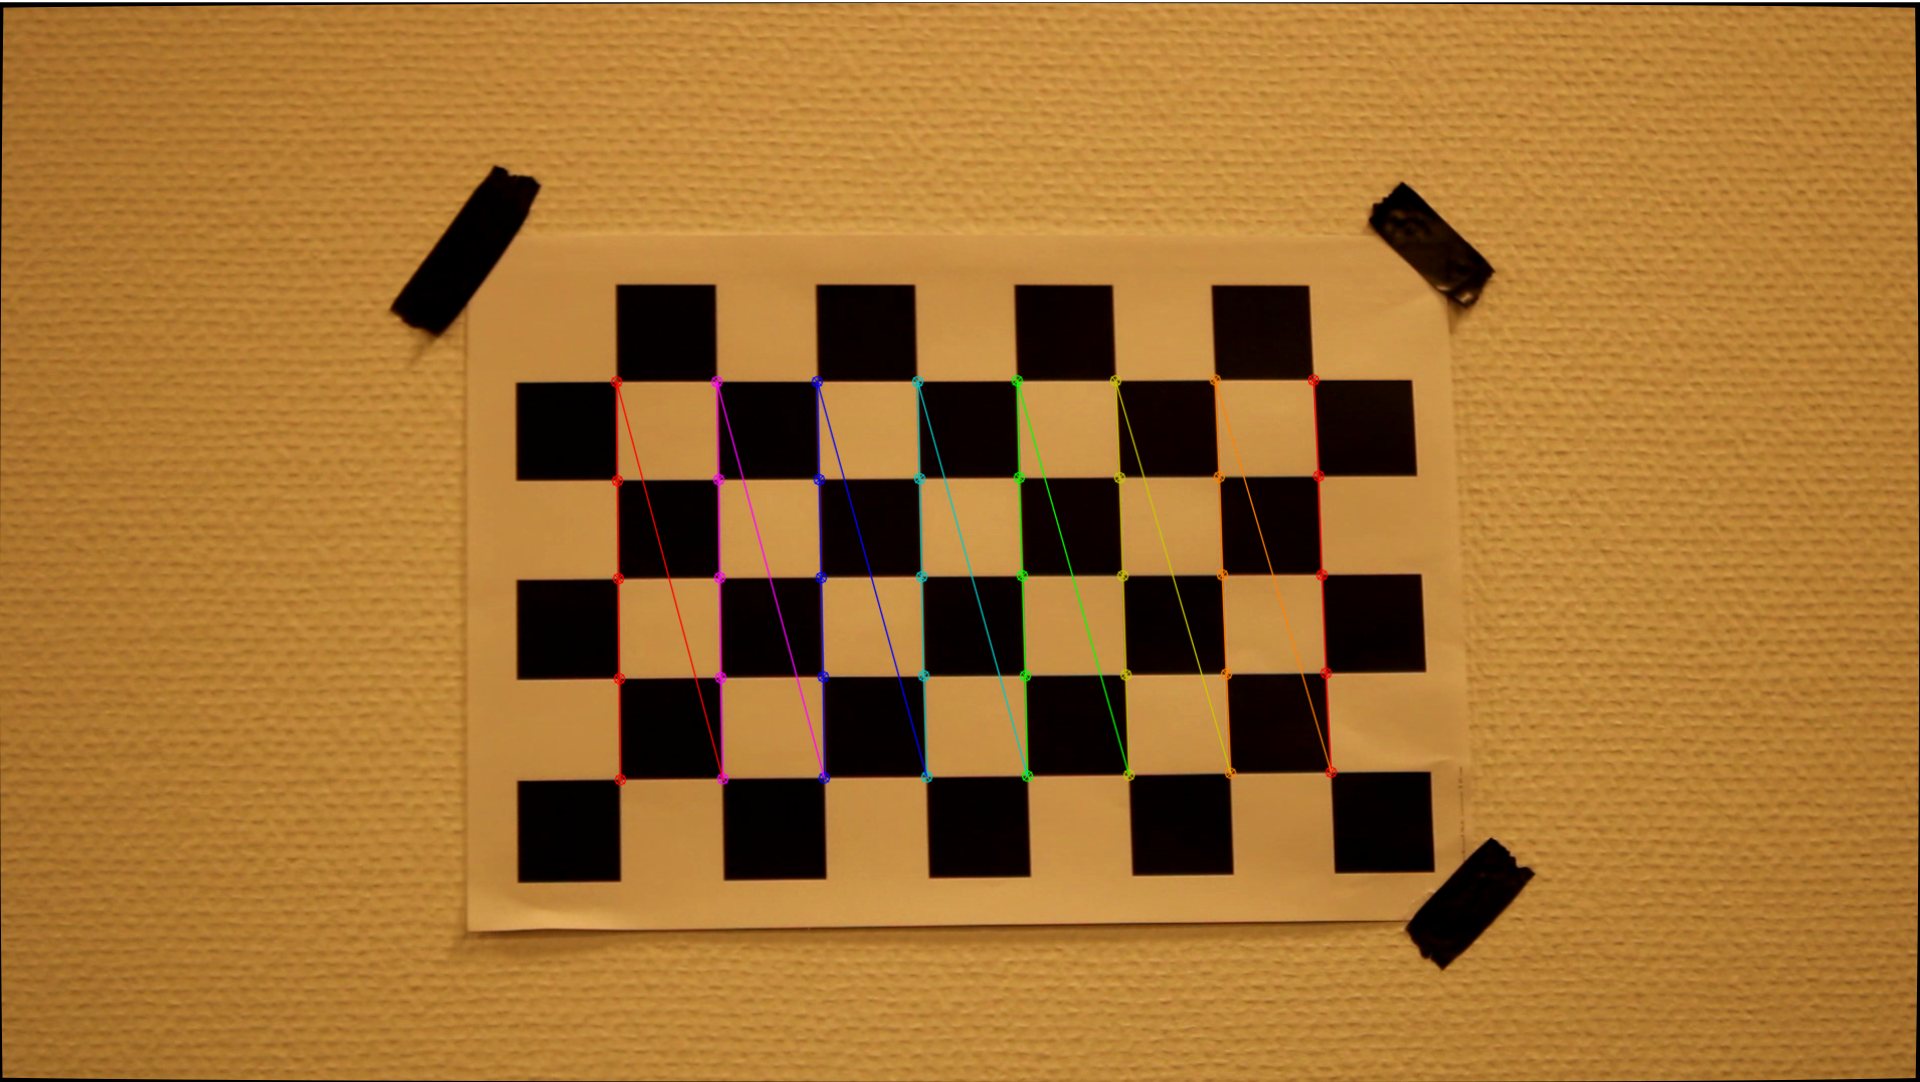
\includegraphics[width=0.95\textwidth]{figures/CameraCalibration/im1_marked_undistorted.png}
        \caption{Undistortion of image from figure \ref{fig:calibpattern1marked}}
    \label{fig:calibpattern1undistorted}

\end{figure}
\FloatBarrier
The undistortion is primarily visible in the corners where there now is a bit of black background due to the image being mapped slightly differently. There was hardly any distortion in the original images, so it makes sense that there is no noticeable difference. \\

Overall the calibration is succesful, but undistortion of the images is deemed unnecessary, as there is very little distortion in the first place. Therefore, undistortion of the data collections will not be done, as this will complicate the process unnecessarily.  


\subsection{Camera calibration routine} 
% basicly just describe what we did, and in sort of a recipe-like fashion
Each time a data collection is done anew, the calibration of the camera must be redone. The details of the calibration have been described above, the actual step-by-step routine is described here. \\

After collecting data, a chessboard pattern is mounted on the wall. For this project, this was the easiest way to fix either the camera or the pattern and get good footage. The pattern must be printed in an appropriate size, such that the camera can capture the pattern in focus, without changing any settings on the camera. This is crucial because the parameters of the calibration will change if the zoom is changed. Changing ISO and shutter speed might not change the actual parameters, but it can make it harder to detect corners and thereby impact the resulting calibration.
\\

The pattern is filmed from many different angles, making sure to keep the pattern in focus at all times. Afterward, the videos are uploaded to a laptop/microcomputer, and the calibration software can be run. The best result is found if a user selects the best frames from the calibration video, but you can also just calibrate based on every 10th frame or the like if you wish to automate your system entirely.\\

The intrinsic, extrinsic, and distortion parameters are then derived and exported, ready to be used in the next program. Here the parameters will be used to undistort the pixels of interest and derive the correct depth of the object that was scanned, hopefully creating a nice 3D point cloud of the object.\\ 

The code for performing camera calibration is attached in appendix \ref{appendixA}. How to extract the dots from the video, and the image analysis methods used, will be discussed in the following chapter. 

